% Author: Till Tantau
% Source: The PGF/TikZ manual
\documentclass{article}

\usepackage{tikz}
% \usepackage[legalpaper, landscape, margin=2in]{geometry}
\usepackage[paperheight=14in,paperwidth=13in,margin=1in,heightrounded]{geometry}
\usepackage{amsmath}
\usetikzlibrary{mindmap,trees}
\usepackage{verbatim}
\graphicspath{ {images/} }

\begin{document}
\pagestyle{empty}

\begin{comment}
:Title: CS6601 Artificial Intelligence Mind Map
:Tags: Manual, Mindmap

| Author: Vitaly Parnas
| Source: CS6601 Course Material

\end{comment}

\begin{tikzpicture}[mindmap, grow cyclic, every node/.style=concept,
    concept color=black,text=white,
    level 1/.append style={font=\Large\bfseries,level distance=5cm,sibling angle=60},
    level 2/.append style={font=\small\bfseries,level distance=3cm,sibling angle=60},
    level 3/.append style ={font=\tiny\bfseries},
    AI/.style= {concept, font=\Huge\bfseries},
    ]

    \node [AI] {CS6601 AI\\
\includegraphics[width=2cm,height=3cm,keepaspectratio]{AI}}
    child[concept color=green!50!white,text=black,level distance=9cm] { node {Search\\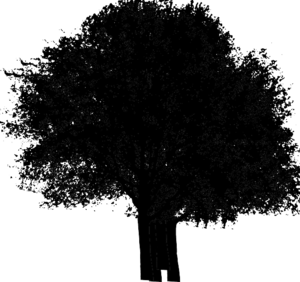
\includegraphics[width=2cm,height=2cm,keepaspectratio]{forest_search}}
        child { node {Completeness} }
        child { node {Optimality} }
        child { node {Uninformed} 
            child { node {Breadth First} }
            child { node {Depth First} }
            child { node {Depth Limited} }
            child { node {Iterative Deepening} }
            child { node {Uniform-Cost} }
            child { node {Bidirectional} }
        }
        child { node {Informed} 
            child { node {$A\star$} }
            child { node {Memory Bounded} }
            child { node {Heuristic} }
        }
        child { node {Local Search} 
            child { node {Hill Climbing} }
            child { node {Simulated Annealing} }
            child { node {Local Beam Search} }
            child { node {Genetic Algorithms} }
        }
        child { node {Constraint Satisfaction} 
            child { node {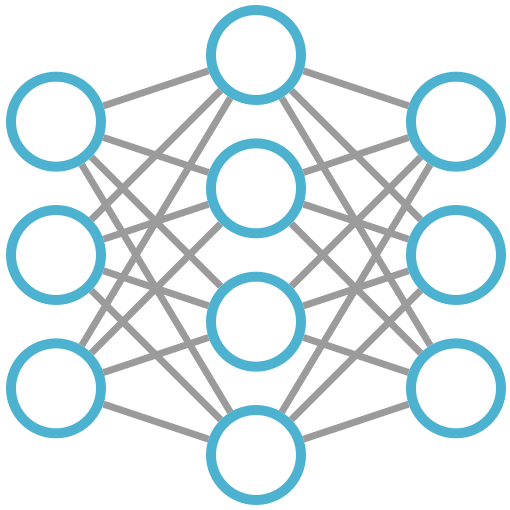
\includegraphics[width=1cm,height=1cm,keepaspectratio]{hypergraph}\\Hypergraph} }
            child { node {Backtracking Search} }
            child { node {Arc Consistency} }
            child { node {Forward Checking} }
        }
    }
    child[concept color=blue!50!white,text=black,level distance=6cm] { node {Games\\
\includegraphics[width=2cm,height=2cm,keepaspectratio]{chess}}
        [counterclockwise from=-45]
        child { node {deterministic} }
        child { node {non-deterministic} }
        child { node {Perfect Info} 
            [counterclockwise from=30]
            child { node {Mini\-Max} 
                [counterclockwise from=-30]
                child { node {$\alpha-\beta$ pruning} }
                child { node {Eval Function} }
                child { node {Quiescence Search} }
                child { node {Horizon Effect} }
            }
            child { node {Expect Mini\-Max} }
        }
        child { node {Imperfect Info} }
    }  
    child[concept color=orange,text=black,level distance=8cm] { node {
\includegraphics[width=1.5cm,height=1.5cm,keepaspectratio]{dice}\\Uncertainty}
        child { node {Bayes Nets} 
            [counterclockwise from=0]
            child { node {Reachability}
                child { node {Active triplets} }
                child { node {Inactive triplets} }
            }
            child { node {Observability} }
            child { node {Explain-Away effect} }
        }
        child[level distance=4cm] { node {Probability Theory} 
            child { node {Full Joint Distr} }
            child { node {Conditional Prob} }
            child { node {Independence} 
                child { node {Conditional} }
                child { node {Unconditional} }
            }
            child { node {Bayes Rule} }
            child { node {Normalizer} }
        }
        child[level distance=4cm] { node {Planning} 
            child { node {Markov Decision Process} 
                child { node {States} }
                child { node {Actions} }
                child { node {Reward Func} }
                child { node {Value Func} }
                child { node {Bellman Equation} }
            }
            child { node {Partially Observable MDP} 
            }
        }
    }
    child [concept color=orange!50!white,text=black] { node  {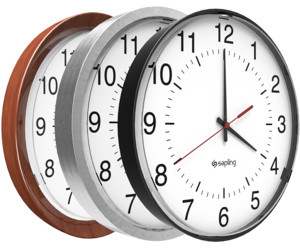
\includegraphics[width=1.5cm,height=1.5cm,keepaspectratio]{clocks}\\Reasoning $\overrightarrow{time}$}
        child { node {Models} 
            child { node {Transition Model} }
            child { node {Markov Chain} }
            child { node {Sensor Model} }
        }
        child { node {Sequence Matching} 
            child { node {Dynamic Time Warp} }
            child { node {Hidden Markov Models} 
                child {node {Trans Prob} }
                child {node {Emission Prob} }
                child {node {Gaussians} }
                child {node {Signal Recognition} }
                child {node {Training} }
            }
            child { node {Viterbi Trellis} }
        }
        child { node {Inference} 
            child { node {Filtering} }
            child { node {Prediction} }
            child { node {Smoothing} }
            child { node {Most\-Likely Exp} }
        }
    }
    child[concept color=pink,text=black,level distance=8cm] { node {Logic\\
\includegraphics[width=2cm,height=2cm,keepaspectratio]{glowing_bulb}}
        child { node {Propositional} 
            child { node {Validity} }
            child { node {Satisfiability} }
            child { node {Variables} }
            child { node {T/F} }
        }
        child { node {First Order} 
            child { node {Model} 
                child { node {Objects} }
                child { node {Constants} }
                child { node {Functions} }
                child { node {Relations} }
            }
            child { node {Syntax} 
                [counterclockwise from=30]
                child { node {$\land \lor \neg \implies \iff ()$} } % Operators
                child { node {$\forall \exists$} } % Quantifiers
            }
        }
        child { node {High Order} }
    }
    child[concept color=red!50!white,text=black] { node {ML\\
\includegraphics[width=2cm,height=2cm,keepaspectratio]{machine_learning}}
        child[level distance=4cm] { node {Example\-Based} 
            child { node {Cross Validation} }
            child { node {K\-Nearest Neighbors} }
            child { node {Decision Trees} 
                child { node {Entropy} }
                child { node {Information Gain} }
            }
            child { node {Random Forests} }
            child { node {Boosting} }
            child { node {Neural Networks} 
                child { node {Input func} }
                child { node {Activation func} }
                child { node {Multilayer Nets} }
                child { node {Perceptron Learning} }
                child { node {Back\-Propagation} }
            }
            child { node {Support Vector Machines} }
        }
        child[level distance=4cm] { node {Probabilistic Models} 
            [counterclockwise from=0]
            child { node {Gaussian Distribution} 
                child { node {Mean} }
                child { node {Variance} }
                child { node {Standard Deviation} }
            } 
            child { node {Bayes Classifier} }
            child { node {Maximum Likelihood} }
            child { node {K\-Means} }
            child { node {Mixture of Gaussians} }
            child { node {Expectation\-Maximization} }
        }
    }
    ;
\end{tikzpicture}\end{document}
